\section{Método}

\subsection{Datos}
Para entrenar nuestras redes y probar los ataques adversarios y las defensas contra ellos, se emplearon las dos bases de datos más sencillas para procesamiento de imágenes: MNIST y CIFAR-10.

\subsubsection{MNIST}
La base de datos MNIST es un compendio de los dígitos del 0 al 9 en letra manuscrita con 60,000 imágenes para entrenar a distintos sistemas de procesamiento de imágenes y 10,000 imágenes para evaluarlos. Se trata de un subconjunto de imágenes de un conjunto más grande que compiló el National Institute of Standards and Technology (NIST) del Departamento de Comercio los EEUU. Las siglas MNIST database significan Modified NIST database. Es una buena base de datos para probar técnicas de aprendizaje y métodos de reconocimiento de patrones con datos del mundo real empleando un esfuerzo mínimo en preprocesamiento y formato.

De las 10,000 imágenes de evaluación, la mitad fueron escritas por estudiantes de preparatoria y la otra mitad por empleados de la oficina de censos, mientras que de las 60,000 imágenes de entrenamiento, 58,527 de los números fueron escritos por 500 estudiantes y el resto por los empleados.

El tamaño de estas imágenes en blanco y negro fue normalizado a una caja de 20$\times$20 pixeles y se colocó su centro de masa en un campo de 28$\times$28 \cite{lecun2010mnist}. En la Figura \ref{mnist} se muestran algunos ejemplos de estas imágenes.

\begin{figure}[h]
    \centering
    \begin{subfigure}[b]{0.4\textwidth}
        \centering
        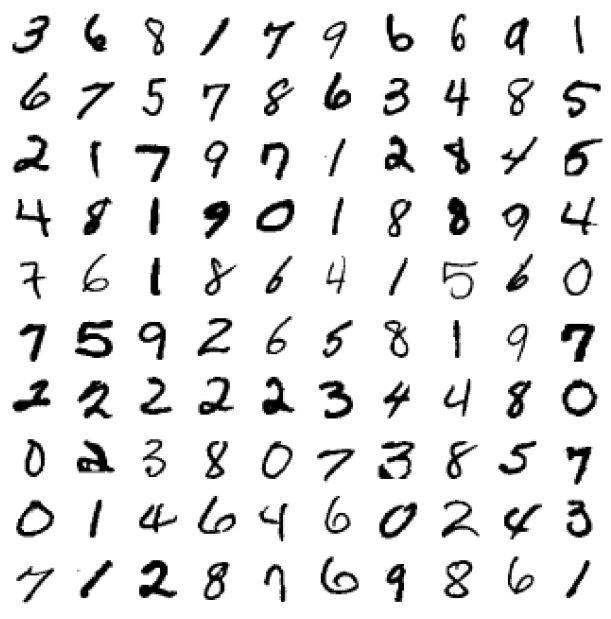
\includegraphics[width=\textwidth]{images/MNIST.png}
        \caption{Algunas imágenes del conjunto de evaluación de la base de datos MNIST \cite{Lecun98}.}
        \label{mnist1}
    \end{subfigure}
    \hspace{1cm}
    \begin{subfigure}[b]{0.45\textwidth}
        \centering
        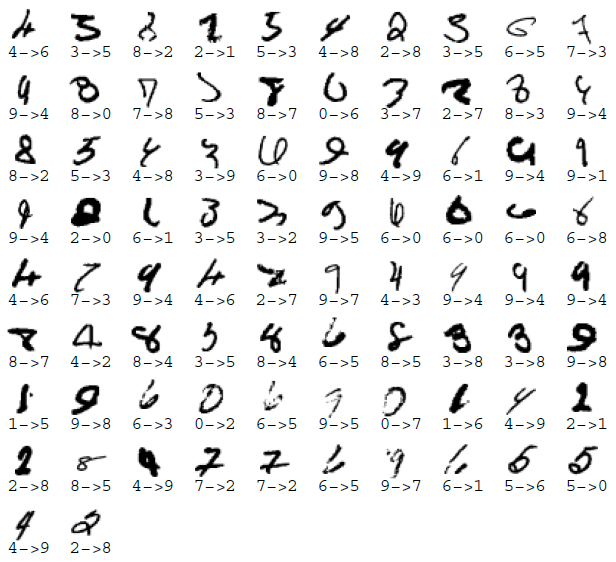
\includegraphics[width=\textwidth]{images/MNISTmiscl.png}
        \caption{82 imágenes de evaluación que LeNet-5 clasificó erróneamente \cite{Lecun98}.}
        \label{mnist2}
    \end{subfigure}
    \caption{Imágenes de MNIST.}
    \label{mnist}
\end{figure}

\subsubsection{CIFAR-10}
Los grupos del MIT y la NYU recopilaron un conjunto de millones de diminutas imágenes en color de la web, se trata de un excelente conjunto de datos para el entrenamiento no supervisado de modelos generativos profundos. Se crearon dos juegos de etiquetas confiables: el conjunto CIFAR-10, que tiene 6000 ejemplos de cada una de 10 clases y el conjunto CIFAR-100, que tiene 600 ejemplos de cada una de 100 clases que no se superponen. Usando estas etiquetas, se mostró que el reconocimiento de objetos mejora significativamente al entrenar previamente una capa de características en un gran conjunto de imágenes diminutas sin etiquetar.

Esta base de datos fue ensamblada buscando en la web imágenes de cada sustantivo en inglés no abstracto en la base de datos léxica WordNet. Utilizaron varios motores de búsqueda, incluidos Google, Flickr y Altavista y mantuvieron aproximadamente los primeros 3000 resultados para cada término de búsqueda. Después de recopilar todas las imágenes para un término de búsqueda en particular, eliminaron duplicados perfectos e imágenes en las que una parte excesivamente grande de los píxeles eran blancos, ya que tendían a ser figuras sintéticas en lugar de imágenes naturales. El término de búsqueda utilizado para encontrar una imagen le proporciona una etiqueta aproximada, aunque es extremadamente poco confiable debido a la naturaleza de la tecnología de búsqueda de imágenes en línea. En total, el conjunto de datos contiene 80 millones de imágenes en color reducidas a 32×32 y distribuidas en 79,000 términos de búsqueda \cite{Krizhevsky09learningmultiple}.

\begin{figure}[h!]
    \centering
    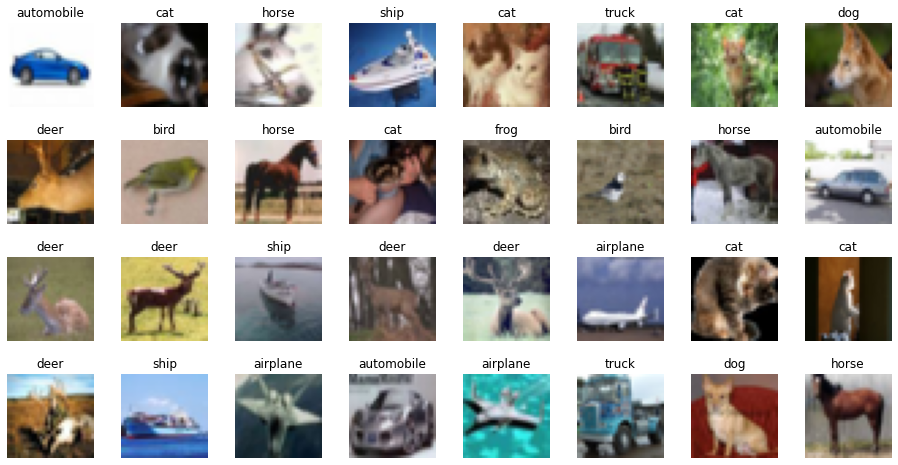
\includegraphics[width=\textwidth]{images/cifar10example.png}
    \caption{Algunas imágenes del conjunto de CIFAR-10 \cite{Krizhevsky09learningmultiple}}
    \label{cifar}
\end{figure}

El conjunto de datos se divide en cinco lotes de entrenamiento y un lote de prueba, cada uno con 10,000 imágenes. El lote de prueba contiene exactamente 1000 imágenes seleccionadas al azar de cada clase. Los lotes de entrenamiento contienen las imágenes restantes en orden aleatorio, pero algunos lotes de entrenamiento pueden contener más imágenes de una clase que de otra. Entre ellos, los lotes de entrenamiento contienen exactamente 5000 imágenes de cada clase \cite{cifarsite}. 

Las 10 clases de CIFAR-10 se encuentran en orden alfabético y son:
\begin{multicols}{5}
\begin{enumerate}
    \item airplane
    \item automobile
    \item bird
    \item cat
    \item deer
    \item dog
    \item frog
    \item horse
    \item ship
    \item truck
\end{enumerate}
\end{multicols}


\subsection{Ataques}

\subsubsection{Fast Gradient Method}
\cite{goodfellow2015explaining, maybe more}

Sean $\theta$ los parámetros de un modelo, $x$ la entrada, $y$ las salidas asociadas, y $J(\theta, x, y)$ la función de costo. La función de costo se lineariza alrededor del valor actual de $\theta$. Sea $\epsilon \in \mathbb{R}^+$. Definamos la imagen adversaria 
\[\tilde{x} = x + \epsilon \eta_{\text{opt}}\]
Se puede definir $\eta_{\text{opt}}$ por el problema de optimización
\[\eta_{\text{opt}} = \operatornamewithlimits{argmax}_{\eta}\left\{ \operatorname{grad} ^\top \eta: \norm{\eta}_p< \epsilon\right\}\]
Donde $p \in \mathbb{N} \cup \{\infty\}$ y $\operatorname{grad} = \nabla_x J(\theta, x, y)$. Experimentamos con tres valores de $p$:
\begin{enumerate}[a)]
    \item $p = 1$, no lo sé, pero se encuentra en el codigo
    \item $p = 2$,
    \[\eta_{\text{opt}} = \frac{\operatorname{grad}}{\norm{\operatorname{grad}}}\]
    \item $p = \infty$,
    \[\eta_{\text{opt}} = \operatorname{sign}(\nabla_x J(\theta, x, y))\]
\end{enumerate}

\subsubsection{Carlini \& Wagner}
\cite{carlini2017evaluating} 

\subsection{Defensas}

\subsubsection{Compresión JPEG }
\cite{das2017keeping}